\documentclass{article}

% Math formulas
\usepackage{amsmath}

%include code
\usepackage{minted}

\usepackage{graphicx}

% Zeichenkodierung und Schriftart
\usepackage[utf8]{inputenc}
\usepackage[T1]{fontenc}
\usepackage{lmodern}

% TikZ
\usepackage{tikz}
\tikzset{
  level/.style={
    sibling distance=40mm/#1
  },
  level distance=10mm,
}

 \tikzset{
  every node/.style={
    draw,
    circle,
    inner sep=0pt,
    minimum width=15pt
  },
  thick
}


\begin{document}
\title{Dynamic Programming}
\author{Juan Andrés Osorio Escobar}
\date{\today}
\maketitle


%include: fügt zeilenumbrüche davor und dahinter: besser geeignet für eigenständige Kapiteln
%input: fügt das nur so ein.

\begin{abstract}
Dynamic Programming (short \textbf{\emph{DP}}) refers to a problem solving paradigm,
  which seeks to solve a problem by solving related subproblems and combining their solutions to solve the main problem.
  As these subproblems may be encountered repeatedly along the solving process, DP algorithms store their solution, so 
  that the same computation is never done twice, potentially making the computation for the main solution much faster at 
  the cost of increased memory usage. DP is often applied to solve optimization problems and counting problems.

  In order for a problem to be applicable to optimization it must exhibit the following traits:

  \begin{itemize}
    \item \textbf{Optimal substructures}: The solution for a subproblem is part of the solution of the original problem \cite{halim2013competitive}.
    \item \textbf{Ovelapping subproblems}: When a recursive algorithm repeatedly revisist the same subproblem in different branches along its recursion tree, we say that the problem has overlapping subproblems \cite{cormen2009introduction}. This is the key characteristic
    which allows the search space for a problem to be drastically reduced \cite{halim2013competitive}.
  \end{itemize}
  
  When these DP criteria are met, DP solutions may reduce the run time of a problem from exponential 
  time complexity (using complete search algorithms), to polynomial time complexity. DP algorithms can be implemented
  in one of two ways: either recursively/top-down with memoization, or bottom-up. Both methods make use of a table in which the solution to subproblems are stored.
  We shall revisit also both techniques and analyze their pros and cons.

  
  
\bibliographystyle{acm}
\bibliography{references.bib}
  
\end{abstract}

\tableofcontents

 
 \section{introduction}


What is dynamic programming? it really sounds like one of those big buzzwords that seem to
attract big audiences that tend to follow trends. But put in simple words, Dynamic Programming is just a tabular method, 
which reduces a lot of duplicate computations on a problem.How does dynamic programming work? lets have a look at an example first: The fibonacci numbers,
which form a sequence defined as follows:

  \[
    fib(n) = \left\{\begin{array}{lr}
      n, & \text{for } n = 1, n = 2\\
      fib(n-1) + fib(n-2), & \text{otherwise}
      \end{array}\right\}
  \]

we could write a simple program to compute the nth fibonacci number as follows:

\begin{minted}[mathescape, linenos]{python}

def fibonacci(n):
  if (n <= 1):
    return n
  else :
    return fibonacci(n - 1) + fibonacci(n + 2)

\end{minted}


to get a rough picture of the space complexity for this program, we could depict the steps
the program would take to compute an arbitrary number n, in the form of a tree. For n = 6, we have:


\begin{figure}[ht]
  \centering
  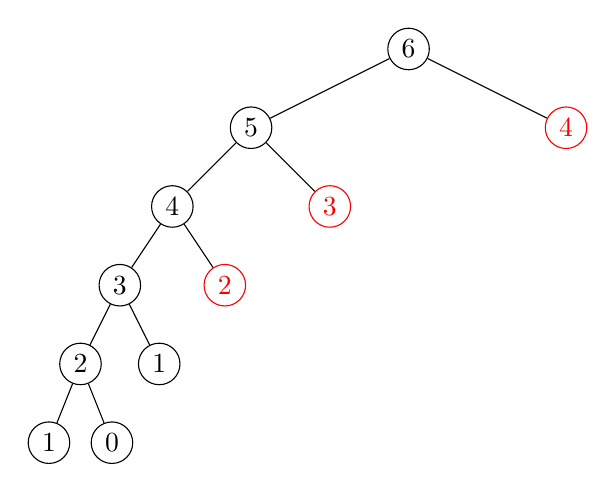
\begin{tikzpicture}
    \node {6}
      child { node {5}
        child { node {4} 
          child{ node {3} 
            child { node {2}
              child {node {1}}
              child {node {0}}
            }
            child { node {1}}
          }
          child{ node[color=red] {2} }
        }
        child { node[color=red] {3} }
      }
      child { node[color=red] {4}
      };
  \end{tikzpicture}
  \caption{Fibonacci recursion tree with $n = 6$}
  \label{fig:fib1}
\end{figure}

There are 6 levels in this call tree and although the red nodes in \autoref{fig:fib1} are 
not expanded, the algorithm has still to do all the work and visit this nodes until it gets to a node
labeled with one or with zero. We can easily see how this can get out of hands with higher numbers, the 
number of nodes is $O(2^n)$

\section{elements of dynamic programming}


\subsection{Optimal substructures}
\section{Matrix-Chain Multiplication}

The Matrix-Chain Multiplication problem is another example in which we can 
apply Dynamic Programming, yielding important performance gains.

Suppose we have a product (also called chain) of Matrices, numbered from 1 to n. Their product is
calculated as follows:

$$A_1A_2A_3...A_n$$

The number of scalar multiplications that have to be performed when multiplying matrices $A_1$
and $A_2$ with dimensions $m_1 \times n_1$ and $m_2\times n_2$ is equal to $m_1*n_1*n_2$ .Rremember that
for a two matrices, rows and columns must match in their number, else the matrices are not 
compatible and the multiplication can not be performed, hence we could have also written $m_1*m_2*n_2$

The product obtained by this multiplication will not vary with the way we parenthesize,
but the ammount of multiplications required may very well vary. Suppose we have
matrices of dimensions $A_1 = 3 \times 50$, $A_2 = 50 \times 2$ and $A_3 = 2 \times 40$, 
the first parenthesization $((A_1A_2)A_3)$ yields $3*50*2 + 3*2*40 = 540$
multiplications, while the second variant $(A_1((A_2A_3))$ yields 
$50*2*40 + 3*50*40 = 10000$ multiplications, an almost scandalous difference.
How we parenthesize a chain of matrices can have a dramatic impact of evaluating
the product \cite{cormen2009introduction}

Now, how does this problem relate to Dynamic Programming? as we just said, in matrix 
multiplication, the way we parenthesize does not alter the end product, in other words it is
\emph{associative}, meaning:  $((A_1A_2)A_3) = (A_1((A_2A_3))$. By using Dynamic Programming
we can abuse the nature of this problem and find an optimal parenthesization.

This problem clearly posseses the property of optimal substructures, an optimal 
parenthesized product consists as well of optimal parenthesized products. An optimal
parenthesized product would be the parenthesization resulting in the minimum of 540
multiplications in our previous example. Suppose instead of having matrices $A_1$, 
$A_2$ and $A_3$ we had products of matrices, which in turn must be optimally parenthesized
to yield an optimal solution.

the abridged problem statement can be written down as follows: given a n chain of matrices,
find a parenthesization with the least ammount of multiplications. These matrices are compatible
for multiplication, and for $i = 1, 2, ..., n$ the matrix $A_i$ has dimension $p_{i-1} * p_i$


In order to better understand the search space for this problem, let us first count the number
of ways we can parenthesize a matrix chain. in \cite{cormen2009introduction}, the number of
parenthesizations of a sequence of n matrices are denoted by P(n). When n = 1, there is just one matrix and there is only
one way to parenthesize it. when $n \geq 2$, a fully parenthesized matrix chain is the product of to 
fully parenthesized subproducts, and the split between two products may occur between the \emph{k}th and the
\emph{(k + 1)}st matrices for any k = 1, 2, ..., n-1. obtaining:
  \\
  \[
    P(n) = \left\{\begin{array}{lr}
      1, & \text{if } n = 1,\\
      \sum_{k=1}^{n-1}P(k)P(n-k), & \text{if } n \geq 2.
      \end{array}\right\}
  \]
  \\


The solution to this recurrence is $\omega (2^n)$ 

DP:
new algo description
complexity new algo


new algo graphics
\section{Solving Dynamic Programming Problems}

A general way to solve Dynamic Programming problems, as seen in \cite{cormen2009introduction}:

\begin{enumerate}
  \item Characterize the structure of an optimal solution.
  \item Recursively define the value of an optimal solution.
  \item Compute the value of an optimal solution, typically in a bottom-up fashion.
  \item Construct an optimal solution from computed information.
\end{enumerate}

\subsection{State and Recurrences}
\section{Dynamic Programming in Programming Contests}

\subsection{Classical Problem Types}

\subsubsection{Knapsack Problem}

\subsubsection{Coin Exchange}
\section{Top-down vs Bottom-up}

We have seen that two common ways to apply Dynamic Programming are using the top-down approach with memoization
and the bottom-up method. Each of these have their own pros and cons. 


\bibliographystyle{acm}
\bibliography{references.bib}

\end{document}